\documentclass[10pt,a4paper]{article}

\usepackage[utf8]{inputenc}
\usepackage[T1]{fontenc}
\usepackage[english]{babel}
\usepackage[margin=1.4cm]{geometry}
\usepackage{enumitem}
\usepackage{microtype}
\usepackage{xcolor}
\usepackage{amsmath}
\usepackage{amssymb}
\usepackage{booktabs}
\usepackage{tabularx}
\usepackage{graphicx}
\usepackage{tikz}
\usepackage[most]{tcolorbox}

\pagestyle{empty}
\setlength{\parindent}{0pt}
\setlength{\parskip}{3pt}

\setlist[itemize]{leftmargin=*, topsep=1pt, itemsep=1pt, parsep=0pt}
\setlist[enumerate]{leftmargin=*, topsep=1pt, itemsep=1pt, parsep=0pt}

\definecolor{groupcolor}{HTML}{24566B}
\definecolor{nnmcolor}{HTML}{4779C4}
\definecolor{torchcolor}{HTML}{C0562F}
\definecolor{arrowcolor}{HTML}{D03B3B}

% Task heading: number, title, right-aligned note.
\newcommand{\task}[3]{%
    \par\medskip
    {\color{groupcolor}\large\bfseries #1\quad #2\hfill\normalfont\footnotesize #3}\par
    \smallskip}

\tcbset{boxrule=0.5pt, arc=1pt, left=4pt, right=4pt, top=2pt, bottom=2pt, fonttitle=\small\bfseries}
\newtcolorbox{nnm}[1][In NNModelling]{colback=nnmcolor!6, colframe=nnmcolor, title={#1}}
\newtcolorbox{torch}{colback=torchcolor!6, colframe=torchcolor, title={In PyTorch (Google Colab)}}

\newcommand{\pkg}[1]{\textsf{#1}}
% Box where the facilitator writes the participant's numeric ID.
\newcommand{\idbox}[1]{\fbox{\rule[-6pt]{0pt}{20pt}\small\bfseries #1:\hspace{3.2cm}}}
\newcommand{\code}[1]{\texttt{\detokenize{#1}}}
\newcommand{\key}[1]{\tikz[baseline=(k.base)]\node[draw=black!50, rounded corners=1.5pt, inner sep=1.5pt, font=\footnotesize\ttfamily](k){#1};}

\begin{document}
\small

{\Large\bfseries Tasks — Expert participants}\ {\footnotesize NNModelling usability study}\hfill\idbox{Participant ID}

\vspace{4pt}\hrule\vspace{6pt}

You will build the same two models twice: once in NNModelling and once in
PyTorch, in the order given by the facilitator. Each task has a tool-neutral
specification, followed by a short note for each tool: read only the box of
the tool you are using. Models are \emph{not} trained.

\begin{itemize}
    \item \textbf{Data.} MNIST small: images \(x\in\mathbb{R}^{B\times1\times28\times28}\)
    (pixels in \([0,1]\)) and integer class targets \(y\in\{0,\dots,9\}^{B}\).
    The dataset is already selected (NNModelling) or loaded (PyTorch).
    \item \textbf{Each task starts from a prepared file}: in NNModelling open the project
    \texttt{projects/taskN-\ldots}; in PyTorch open the Colab notebook from the link the
    facilitator gives you and \textbf{run its first cell before anything else}: type your participant
    number (the box at the top of this sheet), then \(\blacktriangleright\) (it starts the timer). Parts marked as
    \emph{provided} are already there.
    \item \textbf{Submitting.} When you think the model is complete, submit it.
    \textbf{A submission is final}, and neither tool tells you whether it is correct.
    In NNModelling: save the project (\emph{File \(\rightarrow\) Save}). In PyTorch: in the
    \emph{Submit} section, remove the \texttt{\#} at the start of the code line and run that
    cell once. Then tell the facilitator.
    \item \textbf{Same building blocks in both tools.} Use only the operations
    in the table below: no ready-made attention or transformer layers.
\end{itemize}

\begin{nnm}[Moving around in NNModelling]
\begin{minipage}[c]{0.45\linewidth}
\begin{itemize}
    \item \textbf{Move:} click an empty spot of the canvas, then use the arrow keys
    \key{\(\leftarrow\)}\,\key{\(\uparrow\)}\,\key{\(\downarrow\)}\,\key{\(\rightarrow\)}
    (or drag with the middle mouse button).
    \item \textbf{Move several nodes:} drag a rectangle on an empty spot of the canvas
    (or \key{Ctrl}\,+\,click nodes) to select them, then drag one of them: the whole
    group moves.
    \item \textbf{Zoom:} \key{Ctrl}\,+\,\key{+} and \key{Ctrl}\,+\,\key{-}, or the
    \textsf{+} and \textsf{\(-\)} buttons.
    \item \textbf{Fit} shows the whole network; \textbf{Arrange} tidies it
    automatically (use it often).
\end{itemize}
\end{minipage}\hfill
\begin{minipage}[c]{0.53\linewidth}
\centering
\begin{tikzpicture}
    \node[anchor=south west, inner sep=0] (bar) at (0,0)
        {
\includegraphics[width=\linewidth]{img/toolbar.png}};
    \begin{scope}[x={(bar.south east)}, y={(bar.north west)},
                  every node/.style={font=\scriptsize\bfseries, text=arrowcolor},
                  a/.style={-latex, very thick, draw=arrowcolor}]
        \draw[a] (0.34,-0.9) node[below] {Fit} -- (0.34,-0.05);
        \draw[a] (0.49,-1.9) node[below] {zoom in} -- (0.49,-0.05);
        \draw[a] (0.62,-0.9) node[below] {zoom out} -- (0.62,-0.05);
        \draw[a] (0.82,-0.9) node[below] {Arrange} -- (0.82,-0.05);
    \end{scope}
\end{tikzpicture}
\end{minipage}
\end{nnm}

{\footnotesize
\begin{tabularx}{\textwidth}{@{}lXX@{}}
\toprule
Operation & NNModelling package & PyTorch \\
\midrule
Reshape to vectors / rows & \pkg{Flatten} (\texttt{start\_dim}, \texttt{end\_dim}) & \texttt{torch.flatten}, \texttt{nn.Flatten} \\
Affine map on last dim & \pkg{Linear} (\texttt{in\_features}, \texttt{out\_features}) & \texttt{nn.Linear} \\
Activation, normalisation & \pkg{ReLU}, \pkg{Softmax} (\texttt{dim}) & \texttt{torch.relu}, \texttt{nn.ReLU}, \texttt{softmax} \\
Matrix product, transpose & \pkg{MatMul}, \pkg{Transpose} (\texttt{dim0}, \texttt{dim1}) & \texttt{@}/\texttt{torch.matmul}, \texttt{.transpose} \\
Multiply by a number & \pkg{Scale} (\texttt{factor}): tensor in, tensor \(\times\) factor out & \texttt{*} \\
Sum, concatenation & \pkg{Add}, \pkg{Concat} & \texttt{+}, \texttt{torch.cat} \\
Parallel copies of a block & \pkg{Horizontal Repeat} & loop / \texttt{nn.ModuleList} (or \texttt{view} to split heads) \\
Loss & \pkg{Cross Entropy} \(\rightarrow\) \pkg{Loss Output} & \texttt{F.cross\_entropy} \\
\midrule
\multicolumn{3}{@{}l}{\textbf{Not allowed:} \texttt{nn.MultiheadAttention}, \texttt{F.scaled\_dot\_product\_attention}, \texttt{nn.Transformer*}.} \\
\bottomrule
\end{tabularx}}

% ---------------------------------------------------------------------------
\task{Task 1}{Multi-layer perceptron}{same model as the student group}

Classify the digits with a two-layer perceptron:
\[
x \;\xrightarrow{\text{flatten}}\; \mathbb{R}^{784}
  \;\xrightarrow{\text{Linear}}\; \mathbb{R}^{64}
  \;\xrightarrow{\text{ReLU}}\; \mathbb{R}^{64}
  \;\xrightarrow{\text{Linear}}\; \mathbb{R}^{10}\ (\text{logits}),
\qquad \mathcal{L} = \mathrm{CrossEntropy}(\text{logits}, y).
\]
The logits are the output of the model; the cross-entropy is the loss that
training would minimise.

\begin{nnm}
Input, Output and Loss Output are provided. Find packages in the
\emph{Packages} panel (search or browse) and add them to the graph; draw an
edge by dragging from a node's output handle to another node's input handle;
set parameters in the \emph{Inspector} after selecting a node. Connect the last
Linear to both \pkg{Output} and \pkg{Cross Entropy}, and \pkg{Cross Entropy} to
\pkg{Loss Output} (the target \(y\) is supplied by the dataset automatically).
\end{nnm}
\begin{torch}
Complete \texttt{class MLP(nn.Module)} (\texttt{forward(x)} returns the logits)
and \texttt{compute\_loss(logits, target)} in the \emph{Your model} section. The optional
\emph{Try it} section runs your model on a batch and prints shapes, loss and parameter
count; it does not check your answer. Then submit.
\end{torch}

\clearpage
% ---------------------------------------------------------------------------
\task{Task 2}{Multi-head self-attention with model-wide variables}{parametric model}

Treat each image as a sequence of 28 rows (tokens) of 28 pixels and let the
rows attend to each other with \(h\) attention heads. The width \(d\) and the
number of heads \(h\) are declared once, as variables used by the whole model:
\texttt{d-model} and \texttt{num-heads}.
\begin{enumerate}
    \item \emph{Provided:} rows \(X = \mathrm{flatten}(x, 1, 2) \in \mathbb{R}^{B\times28\times28}\),
    embedding \(H = \mathrm{Linear}_{28\to d}(X) \in \mathbb{R}^{B\times28\times d}\), the residual
    sum, the classifier \(\mathrm{Linear}_{28d\to10}(\mathrm{flatten}(H'))\) and the cross-entropy loss.
    \item \textbf{Your part:} each head \(i = 1,\dots,h\) computes
    \(Q_i = \mathrm{Linear}_{d\to d/h}(H)\), \(K_i = \mathrm{Linear}_{d\to d/h}(H)\),
    \(V_i = \mathrm{Linear}_{d\to d/h}(H)\),
    \[
    A_i = \mathrm{softmax}\!\left(Q_i K_i^{\top} \cdot \tfrac{1}{\sqrt{d/h}}\right)\ \text{(over the last dimension, } A_i\in\mathbb{R}^{B\times28\times28}\text{)},
    \qquad \mathrm{head}_i = A_i V_i \in \mathbb{R}^{B\times28\times d/h}.
    \]
    \item The \(h\) heads are concatenated on the last dimension (\(\mathbb{R}^{B\times28\times d}\)) and
    added to the embedding: \(H' = H + \mathrm{concat}(\mathrm{head}_1,\dots,\mathrm{head}_h)\).
    \item Build it with \(d = 32\), \(h = 4\). When it is complete, \textbf{change the variables to
    \(d = 64\) and \(h = 8\)}: the model must remain valid without any other change.
    Leave these final values.
\end{enumerate}

\begin{nnm}
\begin{enumerate}
    \item \textbf{Variables.} \emph{Model \(\rightarrow\) Manage metavariables}: add \texttt{d-model}
    (type \emph{integer}, value 32) and \texttt{num-heads} (type \emph{integer}, value 4).
    \item \textbf{Heads.} Add one \pkg{Horizontal Repeat} between the embedding and the residual
    \pkg{Add}; it runs \texttt{times} copies of the block it contains and concatenates their
    outputs on the last dimension. \\
    \begin{minipage}[c]{0.62\linewidth}
    Click \textbf{Enter subflow} at the bottom of the node to open it: its Input and Output are
    already there; build \emph{one} head inside. The \emph{Scope} selector (top left, \emph{Root})
    brings you back to the main model.
    \end{minipage}\hfill
    \begin{minipage}[c]{0.34\linewidth}
    \centering
    \begin{tikzpicture}
        \node[anchor=south west, inner sep=0] (n) at (0,0)
            {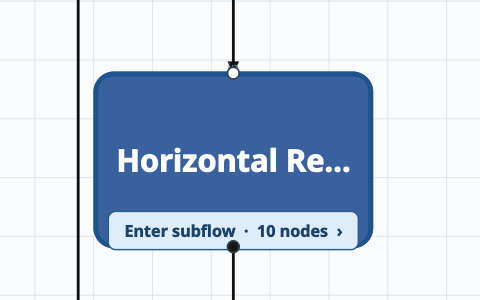
\includegraphics[width=0.6\linewidth]{img/subflow-enter.png}};
        \begin{scope}[x={(n.south east)}, y={(n.north west)}]
            \draw[-latex, very thick, draw=arrowcolor] (1.35,0.22) -- (0.76,0.22);
            \node[font=\scriptsize\bfseries, text=arrowcolor, anchor=south] at (1.15,0.24) {click};
        \end{scope}
    \end{tikzpicture}
    \end{minipage}
    \item \textbf{Inside a head.} \(K_i^{\top}\) is \pkg{Transpose} with \texttt{dim0} \(=-2\), \texttt{dim1} \(=-1\).
    \pkg{MatMul} multiplies its inputs in slot order (\texttt{in-1} \(\times\) \texttt{in-2}), so mind which
    edge goes to which slot. To multiply by \(1/\sqrt{d/h}\) use \pkg{Scale}: connect the tensor
    \(Q_iK_i^{\top}\) to its input; its output is that tensor multiplied by \texttt{factor}, and goes
    into \pkg{Softmax} (\texttt{dim} \(=-1\)). One output may feed several nodes.
    \item \textbf{Parameter values.} Every parameter that depends on \(d\) or \(h\), including those
    of the provided nodes, must be written with the variables, so that the model stays valid
    when they change. A parameter field accepts:\par\smallskip
    {\footnotesize
    \begin{tabularx}{\linewidth}{@{}lXl@{}}
    \toprule
    Form & Meaning & Example \\
    \midrule
    number & a constant & \code{16} \\
    \code{$name} & the value of the variable \texttt{name} & \code{$name} \\
    \code{$(...)} & a Python expression; \code{meta["name"]} is the value of a variable and the
    \code{math} module is available & \code{$(2 * meta["name"] + 1)} \\
    \bottomrule
    \end{tabularx}}
    \item \textbf{Final values.} When the model is complete, set \texttt{d-model} \(=64\) and
    \texttt{num-heads} \(=8\) in \emph{Manage metavariables}, check that the model is still
    valid, then submit.
\end{enumerate}
\end{nnm}
\begin{torch}
Complete \texttt{MultiHeadRowAttentionClassifier(d\_model=32, num\_heads=4)} in the
\emph{Your model} section: the constructor arguments play the role of the variables, and your
submission is checked with \((d,h) = (32,4)\), \((64,8)\) and \((32,2)\). Heads may be separate
modules in a loop or obtained by splitting with \texttt{view}. The embedding, residual,
classifier and loss are provided. Then submit.
\end{torch}

\end{document}
